\chapter{Analysis of Recent Attacks}
\label{ch:AnalysisRecentAttacks}

This chapter presents and analyzes, in chronological order, 
the four \acp{SSCA} that occurred in the \ac{npm} ecosystem in 2025, 
selected as case studies for the metric-based evaluation conducted in \cref{ch:metricsAnalysis}.
Before describing each attack individually, 
\cref{sec:attackModel} introduces the attack model that characterizes all four cases: 
the relevant threat actors, the phases of a typical attack, and the type of artifacts that are modified.
\cref{sec:attackA} through \cref{sec:attackD} then analyze each attack in detail,
describing the number of packages infected, the inner workings,
the characteristics, structure and behavior of the malicious code, 
and the key differences between the compromised versions and their benign counterparts.

\section{Attack Model}
\label{sec:attackModel}

\begin{figure}[htb]
    \centering
    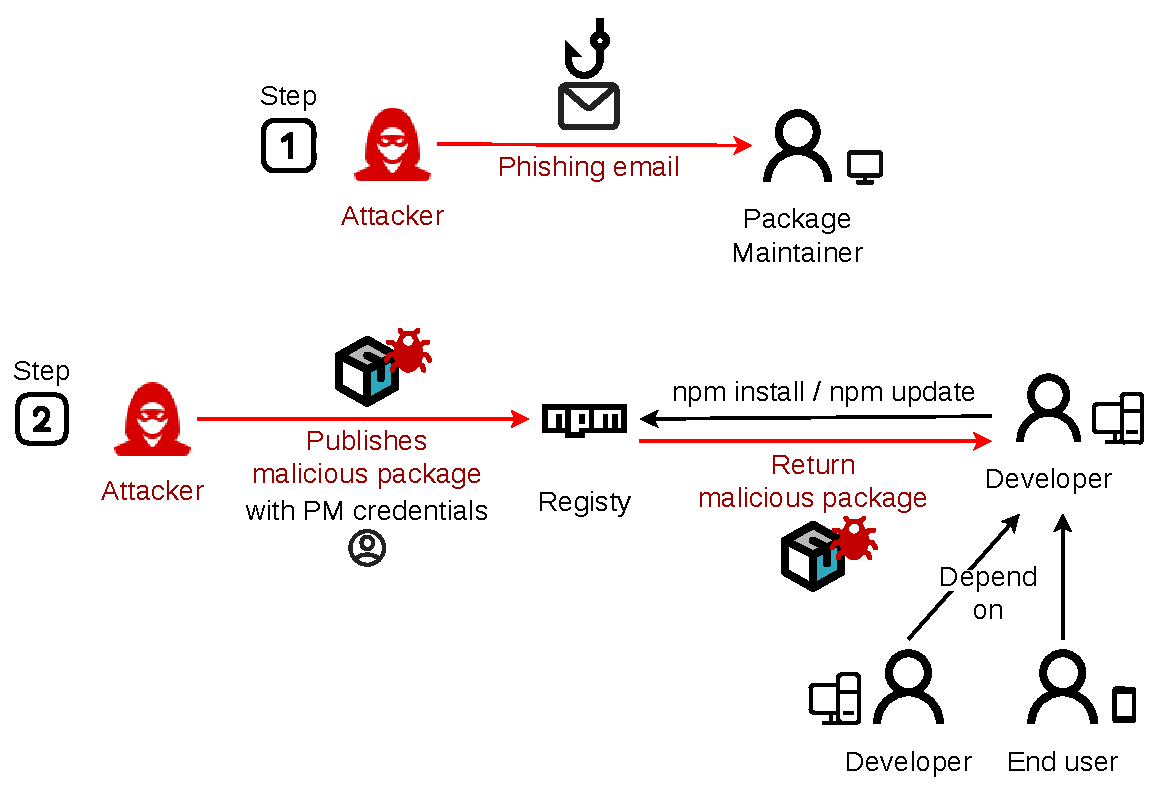
\includegraphics[width=0.90\textwidth]{Attacks/attackModel.pdf}
    \caption{Attack Model for the Four SSCAs.}
    \label{fig:attackModel}
\end{figure}

All four attacks studied in this work follow the same high-level model, illustrated in \cref{fig:attackModel}.
The threat actor is an external attacker who targets the \ac{npm} ecosystem by exploiting the \emph{Account Compromise}:
first, the attacker obtains the credentials of a legitimate \ac{PM}, typically through a phishing campaign (Step~1 in \cref{fig:attackModel}),
and then uses the compromised account to publish a new malicious update of the packages managed by that maintainer (Step~2 in \cref{fig:attackModel}), 
which is automatically distributed to all downstream victims upon the next \texttt{npm install} or \texttt{npm update}.
These include developers who directly depend on the package, those whose projects transitively rely on it,
and end users of the software built on top of it.

The malicious version differs from its legitimate predecessor in the content of the tarball:
the attacker adds one or more new files, or modifies existing ones,
to embed a payload in the tarball, which is automatically activated during installation or update.
The specific payloads differ across the four attacks, as illustrated in \cref{fig:CompromisedPackagePayload}, 
spanning remote code execution via a \acl{DLL} (\cref{sec:attackA}),
cryptocurrency theft through browser transaction hijacking (\cref{sec:attackB}),
and large-scale credential exfiltration with worm-like self-propagation (\cref{sec:attackC,sec:attackD}).

\begin{figure}[htb]
    \centering
    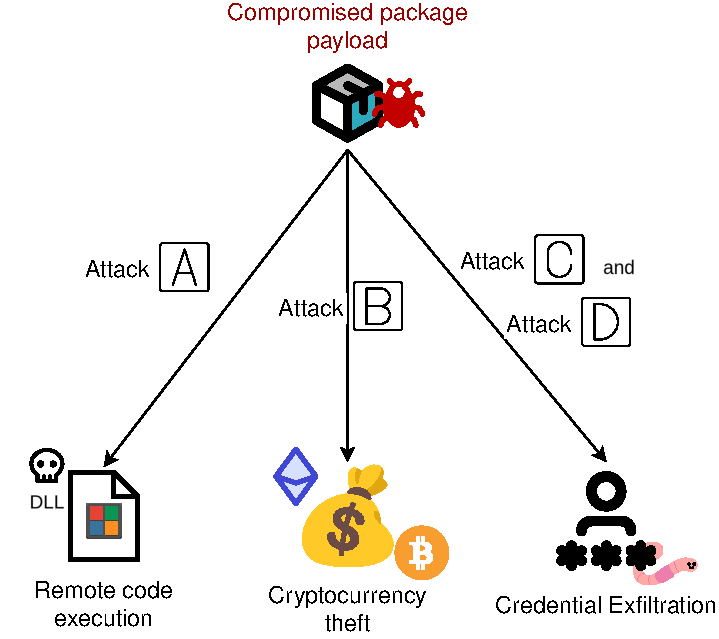
\includegraphics[width=0.67\textwidth]{Attacks/CompromisedPackagePayload.pdf}
    \caption{Compromised Package Payload.}
    \label{fig:CompromisedPackagePayload}
\end{figure}